\documentclass[10pt,twocolumn]{article}
\usepackage{iftex}
\ifPDFTeX
  \usepackage[utf8]{inputenc}
  \usepackage[T1]{fontenc}
  \usepackage{lmodern}
\else
  \usepackage{fontspec}
\fi
\usepackage[spanish,es-tabla,es-nodecimaldot]{babel}
\usepackage[a4paper,margin=1.8cm,columnsep=0.6cm]{geometry}
\usepackage{amsmath,amssymb,bm}
\usepackage{graphicx}
\usepackage{booktabs}
\usepackage{tabularx}
\usepackage{xcolor}
\usepackage{caption}
\usepackage{algorithm}
\usepackage{algpseudocode}
\usepackage{fancyhdr}
\usepackage{titlesec}
\usepackage{natbib}
\usepackage[hidelinks]{hyperref}
\usepackage{xurl}
\captionsetup{font=small,labelfont=bf}
\setlength{\parskip}{2pt}
\titleformat{\section}{\normalfont\large\bfseries}{\thesection.}{0.5em}{}
\titleformat{\subsection}{\normalfont\normalsize\bfseries}{\thesubsection}{0.5em}{}
\titlespacing*{\section}{0pt}{8pt}{3pt}
\titlespacing*{\subsection}{0pt}{6pt}{2pt}
\pagestyle{fancy}
\fancyhf{}
\fancyhead[L]{\small Estadística Bayesiana}
\fancyhead[R]{\small Semestre 4 Año 2026, Grupo 1, páginas \thepage}
\renewcommand{\headrulewidth}{0.4pt}
\fancyfoot[C]{\thepage}
\floatname{algorithm}{Algoritmo}
\renewcommand{\algorithmicrequire}{\textbf{Entrada:}}
\renewcommand{\algorithmicensure}{\textbf{Salida:}}
\newcommand{\logit}{\operatorname{logit}}
\newcommand{\expit}{\operatorname{logit}^{-1}}

\begin{document}

% ------------------------------------------------------------------ PORTADA
\twocolumn[{
\begin{center}
{\small Estadística Bayesiana · Entrega final · Grupo 1 · Proyecto articulado con Pensamiento Crítico en Ciencia de Datos 2}\\[6pt]
{\LARGE\bfseries ¿Dónde y cuándo son más graves los siniestros viales en Bogotá?}\\[3pt]
{\large Severidad relativa por localidad y franja horaria con modelos jerárquicos bayesianos, 2015--2019}\\[5pt]
{\large\itshape Where and when are road crashes more severe in Bogotá? Relative severity by locality and time of day with Bayesian hierarchical models, 2015--2019}\\[8pt]
Jean Paul Rojas Rojas$^{1}$, Daniel Estiven Pacheco Villagrande$^{1,*}$, Diego Andrés Cascante Camacho$^{1}$\\[2pt]
{\small $^{1}$Pregrado Ciencia de Datos, Universidad Externado de Colombia, Bogotá -- Colombia}\\
{\small $^{*}$jean.rojas@est.uexternado.edu.co, daniel.pacheco1@est.uexternado.edu.co, diego.cascante@est.uexternado.edu.co}\\[4pt]
{\small Entrega: 9 de noviembre de 2026}
\end{center}
\vspace{2pt}
\noindent\rule{\textwidth}{0.4pt}
\begin{small}
\noindent\textbf{RESUMEN.} Ordenar las zonas de Bogotá por el número de siniestros que acumulan muestra dónde se concentran, pero no dónde son más graves. Este trabajo estima, para las 80 combinaciones de localidad y franja horaria de Bogotá, la probabilidad de que un siniestro sea grave (con heridos o muertos) y su incertidumbre, con dos modelos jerárquicos bayesianos ajustados por MCMC programado a mano: un Beta-Binomial (Gibbs + Metropolis-Hastings) y una regresión logística con efectos de localidad, franja, interacción y año (Metropolis-Hastings por componentes + Gibbs). Los modelos aprendieron con 101.500 siniestros de 2015--2017 y se validaron una sola vez con 71.943 de 2018--2019. Todas las cadenas convergieron ($\widehat R=1{,}00$, ESS $>8.900$). La severidad va de 18\,\% (Usaquén, tarde) a 55\,\% (Rafael Uribe Uribe, noche). El modelo logístico ordenó el periodo no visto con una correlación de Spearman de 0,93, frente a $-0{,}33$ del orden por número de graves; cumplió los tres criterios de éxito definidos antes de ajustar los modelos (Spearman $\ge0{,}90$, Brier no mayor que el de la proporción cruda, 6 de 10 en el top 10) y sus intervalos predictivos del 90\,\% cubrieron el 95\,\% de las celdas. Ninguna de sus 10 celdas prioritarias está entre las 10 con más siniestros graves: 9 son del sur y 6 de noche. La ganancia frente a la proporción cruda en el orden es pequeña; el aporte principal es una incertidumbre calibrada y estimaciones más estables en celdas pequeñas. Es un prototipo retrospectivo: estima severidad registrada, no riesgo por exposición.
\par\smallskip
\noindent\textbf{Palabras clave:} seguridad vial, severidad relativa, modelo jerárquico bayesiano, Metropolis-Hastings, Gibbs, priorización, Bogotá.
\par\medskip
\noindent\textbf{ABSTRACT.} Ranking areas of Bogotá by the number of crashes they accumulate shows where crashes concentrate, not where they are more severe. We estimate, for the 80 locality $\times$ time-of-day cells of Bogotá, the probability that a crash is severe (injuries or deaths) and its uncertainty, using two Bayesian hierarchical models fitted with hand-coded MCMC: a Beta-Binomial model (Gibbs + Metropolis-Hastings) and a logistic regression with locality, time-of-day, interaction and year effects (component-wise Metropolis-Hastings + Gibbs). The models learned from 101,500 crashes in 2015--2017 and were validated once on 71,943 crashes in 2018--2019. All chains converged ($\widehat R=1.00$, ESS $>8{,}900$). Severity ranges from 18\,\% (Usaquén, afternoon) to 55\,\% (Rafael Uribe Uribe, night). The logistic model ranked the unseen period with a Spearman correlation of 0.93, versus $-0.33$ for ranking by number of severe crashes; it met the three success criteria defined before fitting the models and its 90\,\% predictive intervals covered 95\,\% of cells. None of its 10 priority cells is among the 10 with the most severe crashes: 9 are in the south and 6 at night. The gain over the raw proportion in ranking is small; the main contribution is calibrated uncertainty and more stable estimates for small cells. It is a retrospective prototype: it estimates recorded severity, not exposure-based risk.
\par\smallskip
\noindent\textbf{Keywords:} road safety, relative severity, Bayesian hierarchical model, Metropolis-Hastings, Gibbs sampling, prioritization, Bogotá.
\end{small}
\par\noindent\rule{\textwidth}{0.4pt}
\vspace{6pt}
}]

% ------------------------------------------------------------------ 1
\section{Introducción}
\subsection{Contexto y planteamiento del problema}
Bogotá adoptó la Visión Cero con el Plan Distrital de Seguridad Vial y del Motociclista 2017--2026, que parte de que ninguna muerte en las vías es aceptable \citep{alcaldia2018plan}, y el Plan Distrital de Seguridad Vial 2023--2032 mantiene ese enfoque \citep{bogota2023decreto494}. Entre 2015 y 2020 la Secretaría Distrital de Movilidad (SDM) registró 196.152 siniestros viales \citep{sdm2021datos}. Como no se puede intervenir toda la ciudad a la vez, hay que escoger en qué zonas y horas concentrar controles, señalización y campañas.

Para esa elección no basta con saber dónde se acumulan los siniestros: también importa qué parte de ellos deja víctimas. Este trabajo estima la probabilidad de que un siniestro \emph{registrado} resulte grave (severidad relativa); no estima riesgo, porque la base no trae datos de exposición (la diferencia se explica en la sección~\ref{sec:lit}).

Sobre la priorización actual pudimos documentar que la SDM trabaja con puntos y tramos críticos \citep{sdm2020ficha} y que publica tramos críticos de 2022--2025 definidos por la concentración de peatones, ciclistas y motociclistas muertos y lesionados \citep{sdm2026tramos}. No encontramos un documento que diga cómo se reparten los operativos por zona y franja horaria, y no logramos contacto con la entidad durante el semestre. Por eso no afirmamos cuál es su criterio: usamos el orden por número de siniestros graves como una \emph{referencia de concentración} para comparar.

\subsection{Pregunta de investigación}
\emph{¿Cómo cambia entre las combinaciones de localidad y franja horaria de Bogotá la probabilidad de que un siniestro registrado sea grave, con qué grado de seguridad, y ordenar por esa probabilidad predice mejor la severidad de un periodo no visto (2018--2019) que ordenar por el número acumulado de siniestros graves?}

La pregunta es predictiva: el éxito se mide con un periodo que los modelos no vieron. No busca explicar causas, porque no hay datos de exposición, velocidad ni intervenciones.

\subsection{Justificación}
En la gestión de seguridad vial de otros países, el tamizaje de sitios corrige los conteos crudos acercando los sitios con pocos datos al comportamiento general, porque un sitio puede verse peligroso un año solo por azar \citep{fhwa2014hsm,hauer2002screening}. Este trabajo aplica esa idea a la \emph{severidad}, a una escala en la que se pueden planear operativos (localidad y franja) y con un margen de incertidumbre visible en cada cifra. Los beneficiarios directos serían los equipos que planean controles y campañas; los indirectos, peatones, motociclistas y ciclistas de zonas y horas donde los siniestros dejan más víctimas.

\subsection{Objetivos}
\textbf{General.} Construir un insumo para decidir en qué localidades y franjas concentrar controles, señalización y campañas: un ordenamiento por severidad relativa que declare qué tan segura es cada posición.

\textbf{Específicos.} (1) Describir cómo se reparten los siniestros y los graves por localidad, franja y año, tratando 2020 aparte. (2) Estimar con dos modelos jerárquicos bayesianos, un Beta-Binomial (M1) y una regresión logística (M2), ajustados por MCMC programado a mano, la severidad de las 80 celdas con su intervalo creíble, marcando como no concluyentes las celdas con pocos casos. (3) Comprobar con 2018--2019 si ese orden supera al orden por conteo y a la proporción cruda, con criterios de éxito definidos antes de estimar. (4) Traducir el resultado a tres niveles de prioridad y declarar lo que no permite afirmar; presentarlo a un equipo de la SDM queda como paso siguiente.

\subsection{Estructura del documento}
La sección~\ref{sec:lit} revisa la literatura; la~\ref{sec:eda} presenta los datos, su procedencia y el análisis exploratorio; la~\ref{sec:met}, la verosimilitud, las priors y los algoritmos MCMC; la~\ref{sec:res}, la convergencia, la validación y los resultados; la~\ref{sec:con}, las conclusiones. El apéndice~\ref{sec:apx} contiene las derivaciones. El archivo \texttt{Grupo1\_EntregaFinal\_Bayesiana.py} reproduce todas las cifras y figuras.

% ------------------------------------------------------------------ 2
\section{Revisión de literatura}\label{sec:lit}
Aquí solo resumimos lo que encontraron otros; nuestros resultados empiezan en la sección~\ref{sec:eda}.

\subsection{Conceptos y fundamento teórico}
Hay tres formas de medir la siniestralidad de una zona que se suelen mezclar. La \emph{concentración} es cuántos siniestros se acumulan allí. La \emph{severidad relativa} es qué parte de esos siniestros deja heridos o muertos. El \emph{riesgo} es cuántos siniestros o víctimas hay por cada persona o vehículo que circula, y para medirlo hace falta la exposición (aforos, kilómetros recorridos). Las tres no se mueven juntas: una zona con mucho tráfico puede acumular muchos choques leves sin ser más riesgosa, y otra puede tener pocos registros, pero casi todos con víctimas. \citet{stipancic2019network} lo plantean así: la frecuencia y la severidad son dimensiones independientes del riesgo.

El segundo concepto es la \emph{regresión a la media}: una zona con pocos casos puede verse extrema solo por azar y volver a lo normal en el periodo siguiente. El método bayesiano empírico lo corrige combinando lo observado en cada sitio con lo esperado para sitios parecidos \citep{hauer2002screening}, y el \emph{agrupamiento parcial} de los modelos jerárquicos es su versión bayesiana completa: cada unidad se acerca al promedio de su grupo tanto más cuanto menos datos tiene \citep[cap.~15]{johnson2022bayes}, \citep[cap.~5]{gelman2013bda}. La relación entre ambas ideas orienta el estudio: si se quiere ordenar zonas por severidad, hay que hacerlo sin confundirla con concentración y sin dejarse llevar por las zonas con pocos registros.

\subsection{Antecedentes}
\textbf{Ordenar por concentración.} \citet{chavez2026spatiotemporal} identifican zonas y horas de concentración de accidentes en Ecuador con DBSCAN y series de tiempo, pero miden la concentración de accidentes y de víctimas, no la proporción de graves. La Visión Cero de Nueva York ordena corredores por peatones muertos y heridos graves por milla, e intersecciones por su número \citep{nycdot2023}: usa la gravedad, pero como conteo. \citet{stipancic2019network}, en Quebec, modelan frecuencia y severidad por separado con datos de GPS y flujo; aun así, la correlación entre el orden que predijo su modelo y el de los siniestros observados fue de 0,46 en intersecciones y 0,25 en tramos.

\textbf{Qué se asocia con la gravedad en Colombia.} \citet{cantillo2020exploratory}, con modelos ordenados para tres niveles de severidad en Cartagena, encontraron más probabilidad de siniestro fatal en vías con límite mayor a 40\,km/h, con motocicletas, en hombres y en personas de 60 años o más, y también cerca de puentes peatonales, semáforos y cebras. \citet{vergel2020examining}, con datos de la misma SDM para 2012--2016 en vías arteriales y corredores de TransMilenio, usaron modelos logit ordinales y regresiones, y asociaron la presencia de puentes peatonales con más siniestros, y la densidad y la distancia a intersecciones con la seguridad.

\textbf{El momento del día.} \citet{zeng2023bayesian}, con un modelo bayesiano multivariado con efectos espaciales en 131 zonas de Hong Kong y un año de datos, encontraron que los factores asociados a los siniestros diurnos y nocturnos no son los mismos en cada nivel de severidad. \citet{zou2017truck}, con siniestros de camiones en Nueva York, hallaron que en la tarde y la noche los siniestros de un solo vehículo son menos graves y los de varios vehículos, más graves.

\textbf{Ordenar con pocos datos.} El tamizaje del \emph{Highway Safety Manual} incluye ordenar sitios por la probabilidad de que la proporción de siniestros severos supere un umbral \citep{fhwa2014hsm,fhwascreening}. \citet{lim2013identifying}, con 1.670 intersecciones (2004--2008), encontraron que el método de frecuencia fue el mejor de los tradicionales para identificar el 1\,\% más inseguro, aunque marcó de forma errónea varios de los primeros puntos. \citet{mekonnen2023identifying} aplicaron el bayesiano empírico a tres años de siniestros de Budapest y terminaron con solo tres puntos negros. \citet{dong2016macroscopic}, con zonas de Florida, mostraron que un modelo bayesiano completo con interacción espacio-tiempo identifica mejor los puntos críticos que uno sin efectos de tiempo.

\subsection{Síntesis crítica}
Los estudios coinciden en dos cosas: el lugar y el momento del día cambian la gravedad, y ordenar por frecuencia no es lo mismo que ordenar por severidad. Difieren en cuánto se gana con los métodos bayesianos frente al conteo: \citet{dong2016macroscopic} y \citet{mekonnen2023identifying} muestran ganancias claras, mientras que \citet{lim2013identifying} encuentran que el conteo funciona bien en el extremo superior. Comparten tres limitaciones para nuestro caso: casi todos ordenan \emph{frecuencia} y no proporción de graves; casi todos usan volumen de tránsito, que nuestra base no tiene; y los estudios colombianos explican factores del siniestro individual, varios de los cuales (vehículo, edad de la víctima) solo se conocen después del siniestro, pero no ordenan zonas ni horas. Queda pendiente, entonces, lo que en las fuentes que revisamos no encontramos: un estudio que ordene combinaciones de zona y franja horaria por la \emph{proporción} de siniestros graves, con su incertidumbre y validado en un periodo posterior, con datos administrativos de una ciudad latinoamericana. No decimos que no exista, sino que no apareció en nuestra búsqueda.

\subsection{Conexión con el trabajo}
La literatura sustenta tres decisiones. La \emph{pregunta} mide severidad relativa y la compara con el orden por concentración porque, según \citet{stipancic2019network}, son dimensiones distintas, y porque esa comparación es la que falta en los antecedentes. Las \emph{variables} son localidad, franja y año: \citet{zeng2023bayesian} y \citet{zou2017truck} muestran que el efecto de la franja cambia según el lugar, lo que justifica la interacción localidad $\times$ franja, y los factores de \citet{cantillo2020exploratory} y \citet{vergel2020examining} quedan por fuera como predictores porque solo se conocen después del siniestro. El \emph{método} es un modelo jerárquico con agrupamiento parcial \citep{hauer2002screening,johnson2022bayes}, validado con un periodo posterior y comparado con la proporción cruda y el conteo, porque la evidencia sobre cuánto se gana frente a reglas simples no es uniforme \citep{lim2013identifying,dong2016macroscopic}.

% ------------------------------------------------------------------ 3
\section{Análisis exploratorio}\label{sec:eda}
\subsection{Los datos, su procedencia y disponibilidad}
Usamos la base \emph{Siniestros viales consolidados Bogotá D.C.}, de la SDM, publicada en el portal Datos Abiertos Bogotá (dominio \url{datosabiertos.bogota.gov.co}) \citep{sdm2021datos}. Es el registro administrativo de los siniestros atendidos por las autoridades de tránsito entre el 1 de enero de 2015 y el 31 de diciembre de 2020. Tiene cuatro hojas unidas por el código del siniestro, más un diccionario de códigos: SINIESTROS (196.152 filas: fecha, hora, gravedad, clase, localidad, tipo de lugar), ACTOR\_VIAL (422.416 personas), VEHICULOS (371.605) e HIPOTESIS (233.819 causas probables).

\textbf{Nota sobre la procedencia y disponibilidad de los datos.} Trabajamos con una copia del archivo que el equipo descargó del portal antes de empezar el análisis; la más antigua que conservamos tiene fecha del 12 de agosto de 2026 y la que se usó para correr el código, del 25 de octubre de 2026 (las dos tienen las mismas filas por hoja). Al volver a consultar el portal no pudimos acceder al recurso en las mismas condiciones: el 9 de noviembre de 2026 aparecía como restringido. No tenemos información suficiente para saber por qué, así que no le atribuimos una causa. Para que el análisis se pueda revisar, conservamos y documentamos la versión usada: según sus propiedades internas, el archivo se creó el 8 de abril de 2021 y se modificó por última vez el 21 de octubre de 2021, y la base limpia que se deriva de él (\texttt{siniestros\_limpios.csv}) se entrega con el código. Hoy la SDM publica en su portal de datos la capa \emph{Siniestralidad BD}, con siniestros georreferenciados desde 2007 y actualización diaria \citep{sdmsigat}; no la usamos, pero sería la vía para actualizar este prototipo.

\subsection{Análisis descriptivo}
Cada fila de SINIESTROS es un siniestro y aparece una sola vez; es la unidad de registro. Llamamos \emph{grave} a un siniestro con al menos una persona herida o muerta. En 2015--2019 hubo 173.443 siniestros, 59.303 graves (34,2\,\%) y 2.626 con al menos un muerto. En los campos que usa el modelo (fecha, hora, localidad y gravedad) no hay faltantes. Hay 175 siniestros cuya gravedad contradice el estado de las personas y 24 sin personas asociadas que dicen tener víctimas; se marcan y se usa la gravedad oficial. El 38,9\,\% de las horas está anotado en punto o y media (por azar sería cerca del 3\,\%), por lo que no usamos cortes de menos de tres horas. Sumapaz tiene solo 5 siniestros en cinco años.

\subsubsection*{Procesamiento de los datos}
(i) Respuesta binaria: grave $=1$ si hubo heridos o muertos, $0$ si solo daños. (ii) Franja: madrugada (0--6\,h), mañana (6--12), tarde (12--18) y noche (18--24); como sensibilidad, ocho franjas de tres horas. (iii) \emph{Celda} $c$: cada combinación de localidad y franja ($20\times4=80$), con $n_c$ siniestros y $y_c$ graves; para M2 la celda se abre además por año. Las 80 celdas incluyen las cuatro de Sumapaz, que tuvo 5 siniestros en 2015--2019 y solo 1 en 2015--2017, así que tres de sus celdas quedan vacías en el ajuste. Los modelos las estiman igual, apoyados en el resto de la ciudad, pero se marcan como no concluyentes y no entran a la validación, que usa las 75 celdas con al menos 30 siniestros en ambos periodos (quedan fuera Sumapaz y La Candelaria en la madrugada). Este diseño reemplaza el ejercicio preliminar de 95 celdas (cinco franjas, sin Sumapaz) de nuestro marco teórico. (iv) Partición temporal: el modelo aprende con 2015--2017 (101.500 siniestros) y se prueba una sola vez con 2018--2019 (71.943); 2020 se usa aparte como prueba de ruptura. (v) No entran al modelo clase de siniestro, choque, presencia de moto o peatón, estado de las personas ni causa probable, porque solo se conocen después del siniestro y casi definen la gravedad (fuga de información). (vi) El día de la semana se evaluó y no se incluyó: la proporción de graves va de 33,0\,\% los viernes a 37,3\,\% los domingos, frente a 21,0--52,5\,\% entre localidades; la variación relevante es territorial. (vii) Conforme a la Ley 1581 de 2012, no se usan datos personales de ACTOR\_VIAL y solo se publican agregados por celda.

\subsection{Gráficas}
\begin{figure}[t]
\centering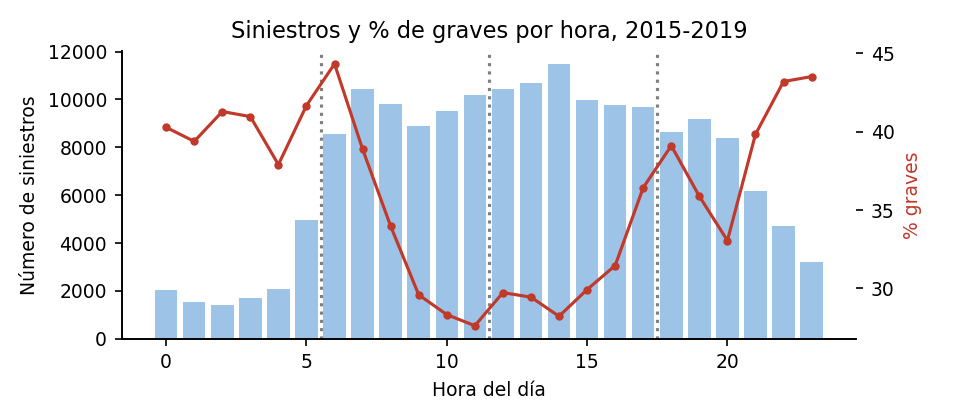
\includegraphics[width=\columnwidth]{figuras/eda_hora.png}
\caption{Número de siniestros (barras) y porcentaje de graves (línea) por hora, 2015--2019. Las líneas punteadas separan las cuatro franjas: la tarde concentra más siniestros, pero la madrugada y la noche tienen más proporción de graves. Fuente: elaboración propia con datos de la SDM \citep{sdm2021datos}.}\label{fig:hora}
\end{figure}
\begin{figure}[t]
\centering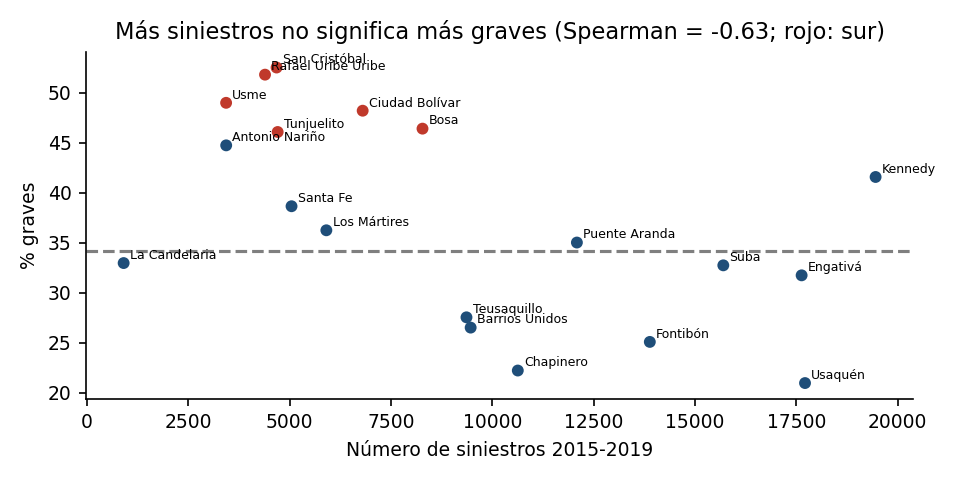
\includegraphics[width=\columnwidth]{figuras/eda_localidad.png}
\caption{Siniestros frente a porcentaje de graves por localidad, 2015--2019 (rojo: localidades del sur; línea: promedio de la ciudad; Sumapaz no se muestra). Fuente: elaboración propia con datos de la SDM \citep{sdm2021datos}.}\label{fig:loc}
\end{figure}
La Figura~\ref{fig:hora} tiene forma de U: entre las 9 y las 16 hay muchos siniestros, pero solo 28--30\,\% son graves; en la madrugada y al final de la noche hay pocos, pero cerca del 40\,\% o más tienen víctimas, lo que coincide con la mayor severidad nocturna que reportan \citet{vergel2020examining} (quienes, en cambio, hallan la mayor probabilidad de muerte entre el mediodía y las 6 p.\,m.). En la Figura~\ref{fig:loc}, las localidades con más siniestros (Usaquén, Engativá, Suba) tienen menor proporción de graves y las del sur (San Cristóbal, Rafael Uribe Uribe, Usme, Ciudad Bolívar) se acercan a la mitad; la correlación de Spearman entre ambas cosas es $-0{,}63$. Puede ser que allí los siniestros sean más graves o que allí se reporten menos los choques leves; por eso una de las sensibilidades usa solo siniestros con muertos, que casi siempre se registran.

\begin{figure}[t]
\centering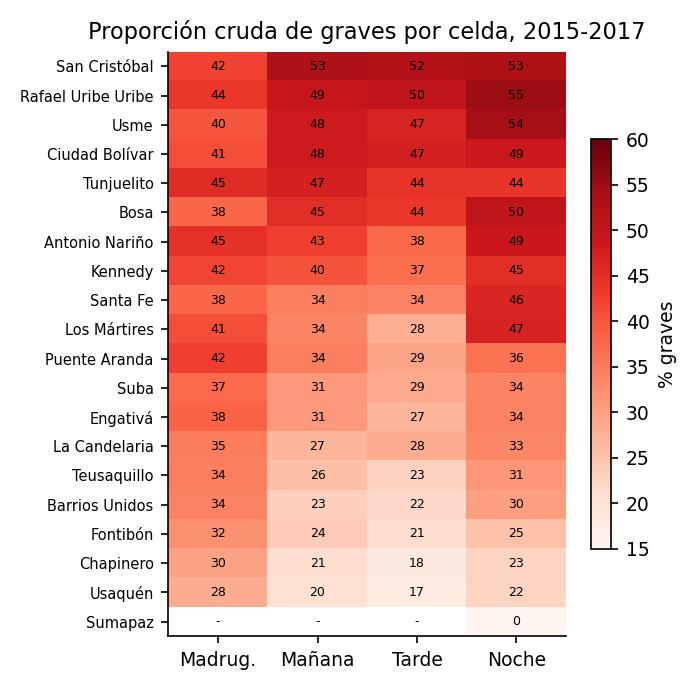
\includegraphics[width=0.92\columnwidth]{figuras/eda_celdas.png}
\caption{Proporción cruda de graves por celda en el periodo de ajuste, 2015--2017. Las localidades están ordenadas de mayor a menor severidad; ``-'' indica celdas sin siniestros (Sumapaz). Fuente: elaboración propia con datos de la SDM \citep{sdm2021datos}.}\label{fig:celdas}
\end{figure}
\begin{figure}[t]
\centering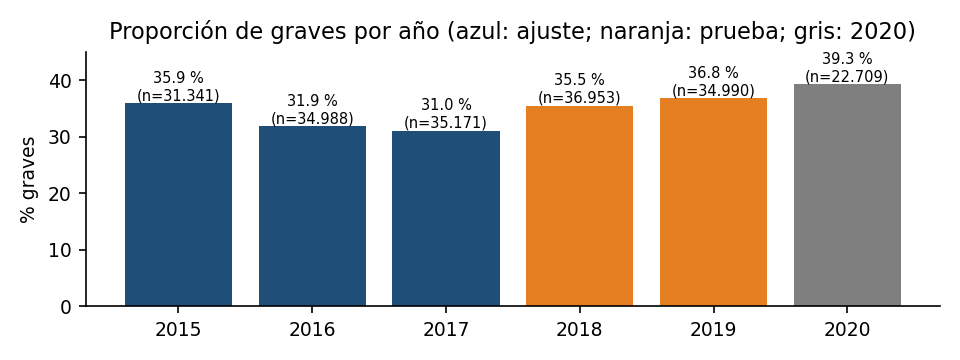
\includegraphics[width=\columnwidth]{figuras/eda_anio.png}
\caption{Proporción de graves por año. El nivel de la ciudad sube de 31--36\,\% en el ajuste a 36--37\,\% en la prueba y a 39\,\% en 2020: el modelo debe ordenar bien aunque el nivel cambie. Fuente: elaboración propia con datos de la SDM \citep{sdm2021datos}.}\label{fig:anio}
\end{figure}
La Figura~\ref{fig:celdas} muestra que la proporción por celda va de 17\,\% a 55\,\% y que la estructura es casi aditiva: una localidad del sur es severa en todas sus franjas y la noche es severa en casi todas las localidades. Las diferencias entre celdas son mucho mayores que las del azar ($\chi^2=4.648$ con 74 grados de libertad) y localidad y franja juntas explican cerca del 95\,\% de ellas. La Figura~\ref{fig:anio} advierte un cambio de nivel entre periodos, que afecta la calibración (Brier) pero no el orden.

\subsection{Hipótesis}
H1: el orden de las celdas por número de siniestros graves no coincide con el orden por proporción de graves; ninguna de las 10 celdas con mayor proporción en 2015--2017 está entre las 10 con más graves. H2: un modelo jerárquico ordena 2018--2019 con Spearman $\geq 0{,}90$, no predice peor que la proporción cruda (Brier $\leq 0{,}2218$, el de la cruda) y logra al menos 6 coincidencias en el top 10. H3: incluir la estructura localidad + franja (M2) mejora a M1 en celdas pequeñas.

% ------------------------------------------------------------------ 3
\section{Metodología}\label{sec:met}
\subsection{Verosimilitud}
La unidad de análisis es el siniestro. Para el siniestro $i$, $Y_i=1$ si fue grave y $0$ si no, con $Y_i\mid\theta_{c(i)}\sim\mathrm{Bernoulli}(\theta_{c(i)})$, donde $c(i)$ es su celda. Suponemos que dentro de una celda todos los siniestros tienen la misma probabilidad de ser graves y son independientes entre sí. Entonces el número de graves de la celda, $y_c=\sum_{i\in c}Y_i$, sigue una Binomial, y su verosimilitud es la de los siniestros uno por uno salvo una constante:
\begin{gather}
y_c\mid\theta_c\sim\mathrm{Binomial}(n_c,\theta_c),\nonumber\\
p(\bm y\mid\bm\theta)=\prod_{c}\binom{n_c}{y_c}\theta_c^{y_c}(1-\theta_c)^{n_c-y_c}.\label{eq:lik}
\end{gather}
En cada celda, el numerador es $y_c$, el denominador es $n_c$ y lo que se estima es $\theta_c$. En M2 la misma verosimilitud se aplica a cada celda-año $(l,f,t)$. Los expertos y la literatura intervienen solo en las priors, no en la verosimilitud.

\subsection{M1: Beta-Binomial jerárquico}
Las severidades de las 80 celdas vienen de una distribución común de la ciudad, con centro $m$ y concentración $\kappa$:
\begin{gather}
\theta_c\mid m,\kappa\sim\mathrm{Beta}\big(m\kappa,(1-m)\kappa\big),\nonumber\\
m\sim\mathrm{Beta}(2,4),\qquad \kappa\sim\mathrm{Gamma}(2,\,0{,}04).\label{eq:m1}
\end{gather}
La media posterior condicional de cada celda es un promedio ponderado (apéndice~\ref{apx:enc}): $E[\theta_c\mid y_c,m,\kappa]=\frac{\kappa}{\kappa+n_c}m+\frac{n_c}{\kappa+n_c}\frac{y_c}{n_c}$; la ciudad ``presta'' $\kappa$ siniestros a cada celda.

\subsection{M2: regresión logística jerárquica}
M1 trata las 80 celdas como intercambiables, pero la EDA mostró que localidad y franja explican casi toda la variación entre celdas. M2 es una regresión logística bayesiana que usa esa información. La respuesta es la misma, $Y_i\sim\mathrm{Bernoulli}(\theta_i)$, y los predictores son indicadoras de la localidad del siniestro (20 categorías), su franja (4), la combinación de las dos y el año (2015, 2016 o 2017), todas conocidas antes del siniestro. Con el enlace logit,
\begin{multline}
\logit\,\theta_i=\log\frac{\theta_i}{1-\theta_i}\\
=\mu+\sum_{l}a_l x_{il}+\sum_{f}b_f z_{if}+g_{l(i)f(i)}+d_{t(i)},\label{eq:m2i}
\end{multline}
donde $x_{il}=1$ si el siniestro ocurrió en la localidad $l$ y $z_{if}=1$ si ocurrió en la franja $f$. Como todos los siniestros de una misma celda y año comparten la misma probabilidad, el modelo se ajusta con los conteos, $y_{lft}\sim\mathrm{Binomial}(n_{lft},\theta_{lft})$, con
\begin{align}
\logit\,\theta_{lft}&=\mu+a_l+b_f+g_{lf}+d_t,\label{eq:m2}\\
\mu&\sim N\big(\logit(1/3),\,1\big),\nonumber\\
a_l&\sim N(0,\sigma_a^2),\quad b_f\sim N(0,\sigma_b^2),\nonumber\\
g_{lf}&\sim N(0,\sigma_g^2),\quad d_t\sim N(0,\sigma_d^2),\nonumber\\
\sigma_a^2,\sigma_b^2&\sim\mathrm{IG}(3;\,0{,}5),\quad \sigma_g^2\sim\mathrm{IG}(3;\,0{,}1),\nonumber\\
\sigma_d^2&\sim\mathrm{IG}(3;\,0{,}05).\nonumber
\end{align}
$\mu$ es el intercepto y $a_l$, $b_f$, $g_{lf}$ y $d_t$ son los coeficientes. En lugar de fijar una categoría de referencia, cada coeficiente se mide frente al promedio y todos los de un mismo grupo comparten una prior normal centrada en cero con varianza desconocida; por eso los coeficientes con pocos datos se encogen hacia cero (agrupamiento parcial). Un coeficiente positivo sube la probabilidad de grave: $e^{b_f}$ es la razón de odds de la franja $f$ frente a la franja promedio, para una localidad típica (sin contar la interacción). Para predecir un año no visto se integra sobre un efecto de año nuevo, $\theta^{\mathrm{nuevo}}_{lf}=\expit(\mu+a_l+b_f+g_{lf}+d^{*})$ con $d^{*}\sim N(0,\sigma_d^2)$, lo que agrega la incertidumbre de un año a otro.

\subsection{Especificación y argumento de las priors}
Ninguna prior usa datos de 2018--2019. La Tabla~\ref{tab:priors} resume distribuciones, hiperparámetros y argumento.
\begin{table*}[t]
\centering\small
\caption{Priors de M1 y M2: distribución, hiperparámetros y argumento. Fuente: elaboración propia.}\label{tab:priors}
\begin{tabularx}{\textwidth}{@{}p{3.3cm}X@{}}
\toprule
Prior & Argumento \\
\midrule
$m\sim\mathrm{Beta}(2,4)$ & Severidad típica de la ciudad. Media $1/3$; 90\,\% central entre 6\,\% y 66\,\%. Débilmente informada por \citet{vergel2020examining} ($\approx$30\,\% con víctimas en 2012--2016); se deja ancha porque ese periodo se solapa con 2015--2016. \\
$\kappa\sim\mathrm{Gamma}(2;\,0{,}04)$ & Cuántos siniestros ``presta'' la ciudad a cada celda. Media 50 y 90\,\% entre 9 y 119: pesa mucho en una celda con 5 casos y casi nada en una con 1.500. Sensibilidad con media 10 y 300. \\
$\mu\sim N(\logit\frac13,\,1)$ (intercepto) & Mismo centro que $m$ en escala logit; 95\,\% entre 7\,\% y 78\,\%. \\
$\sigma_a^2,\sigma_b^2\sim\mathrm{IG}(3;\,0{,}5)$ (coeficientes de localidad y franja) & Media 0,25 ($\sigma\approx0{,}5$): permite que una localidad o franja típica se aleje del centro unos $\pm$11 puntos (de 23\,\% a 45\,\%), coherente con la mayor severidad nocturna que reporta la literatura en vías arteriales. Conjugada, lo que permite un paso de Gibbs. \\
$\sigma_g^2\sim\mathrm{IG}(3;\,0{,}1)$ (interacción) & Media 0,05 ($\sigma\approx0{,}22$): la interacción se espera menor que los efectos principales (principio de jerarquía de efectos). \\
$\sigma_d^2\sim\mathrm{IG}(3;\,0{,}05)$ (año) & Media 0,025 ($\sigma\approx0{,}16$): el nivel anual de la ciudad varía pocos puntos ($\pm$4) de un año a otro. \\
\bottomrule
\end{tabularx}
\end{table*}
Para revisar que las priors son razonables simulamos 4.000 ciudades usando solo las priors y el número real de siniestros por celda en 2015--2017 (Figura~\ref{fig:ppc}). Los cuatro estadísticos observados (media 36,9\,\%, desviación 9,9 puntos, rango 37,7 puntos y 9,3\,\% de celdas sobre 50\,\%) caen entre los percentiles 20 y 83 de lo simulado en ambos modelos: las priors no imponen el resultado, pero tampoco lo descartan.
\begin{figure}[t]
\centering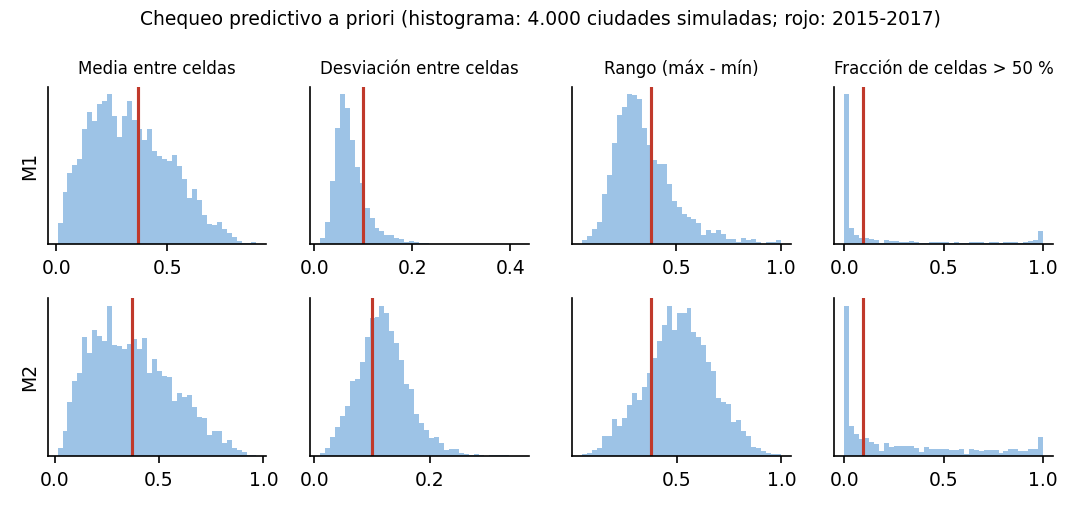
\includegraphics[width=\columnwidth]{figuras/prior_predictivo.png}
\caption{Chequeo predictivo a priori de M1 (arriba) y M2 (abajo): cuatro estadísticos de las celdas con al menos 30 siniestros en ciudades simuladas solo con las priors. Línea roja: valor observado en 2015--2017. Fuente: elaboración propia con datos de la SDM \citep{sdm2021datos}.}\label{fig:ppc}
\end{figure}

\subsection{Algoritmos MCMC}
Ambos muestreadores se programaron a mano en NumPy (sin librerías de MCMC), con 4 cadenas de distinto punto inicial, 5.000 iteraciones de calentamiento ---en las que se adapta la escala de las propuestas hacia una aceptación de 25--44\,\%--- y 20.000 iteraciones guardadas por cadena. ArviZ \citep{kumar2019arviz} se usó solo para calcular $\widehat R$ y el tamaño efectivo de muestra (ESS) \citep{vehtari2021rhat}. Para reproducir: semilla 20261109, Python 3.12.10, NumPy 2.3.5, pandas 2.3.3, SciPy 1.18.1, Matplotlib 3.10.7 y ArviZ 0.23.4; la copia de la base es la descrita en la sección~\ref{sec:eda}. El notebook \texttt{notebooks/Grupo1\_Bayesiana\_completo.ipynb}, ejecutable en Colab, reúne todo el análisis en ocho etapas (carga y limpieza, EDA, del EDA al modelo, priors, M1, M2, validación y sensibilidades); su \texttt{README.md} indica qué celda produce cada cifra y figura de este informe.

\textbf{M1: Gibbs con un paso de Metropolis-Hastings.} Por conjugación Beta-Binomial, la condicional completa de cada $\theta_c$ es Beta y se muestrea exactamente (Gibbs). La de $(m,\kappa)$ no tiene forma conocida y se actualiza con un paseo aleatorio en $(u,v)=(\logit m,\log\kappa)$, incluyendo el jacobiano (apéndice~\ref{apx:m1}).
\begin{algorithm}[t]
\caption{Gibbs + Metropolis-Hastings para M1}\label{alg:m1}
\small
\begin{algorithmic}[1]
\Require $n_c,y_c$; valores iniciales $m^{(0)},\kappa^{(0)}$; escalas $s_u,s_v$
\For{$s=1,\dots,S$}
\State \textbf{Gibbs:} $\theta_c^{(s)}\sim\mathrm{Beta}(m\kappa+y_c,\,(1-m)\kappa+n_c-y_c)$
\State Proponer $u'=u+s_u\varepsilon_1$, $v'=v+s_v\varepsilon_2$, $\varepsilon_i\sim N(0,1)$
\State $\log r=\log\pi(u',v'\mid\bm\theta^{(s)})-\log\pi(u,v\mid\bm\theta^{(s)})$
\State Con probabilidad $\min(1,r)$ aceptar $(u,v)\gets(u',v')$
\State Si $s\le$ calentamiento: ajustar $s_u,s_v$ cada 100 iter.
\EndFor
\Ensure $\{m^{(s)},\kappa^{(s)},\bm\theta^{(s)}\}$; $\log\pi$ en la ec.~\eqref{eq:apx_m1}
\end{algorithmic}
\end{algorithm}

\textbf{M2: Metropolis-Hastings por componentes y Gibbs para las varianzas.} Cada efecto se actualiza con un paseo aleatorio normal. Como, dados los demás parámetros, la condicional de $a_l$ solo depende de las filas de la localidad $l$, los 20 $a_l$ se proponen y aceptan a la vez de forma independiente (lo mismo para $b_f$, $g_{lf}$ y $d_t$). Para romper la correlación entre el intercepto y los efectos, se añaden movimientos de \emph{traslación} ($\mu+c$, $a_l-c$, etc.) que no cambian la verosimilitud y se aceptan solo con la razón de priors. Las varianzas tienen condicional Inversa-Gamma y se muestrean exactamente (apéndice~\ref{apx:m2}).
\begin{algorithm}[t]
\caption{MH por componentes + Gibbs para M2}\label{alg:m2}
\small
\begin{algorithmic}[1]
\For{$s=1,\dots,S$}
\For{bloque $x\in\{\mu,\bm a,\bm b,\bm g,\bm d\}$}
\State $x'_j=x_j+s_j\varepsilon_j$ para cada componente $j$
\State $\log r_j=\sum_{i\in j}[\ell_i(x')-\ell_i(x)]+\log\frac{p(x'_j)}{p(x_j)}$
\State Aceptar cada $x'_j$ con prob. $\min(1,r_j)$
\EndFor
\State Traslaciones $(\mu,\bm a)$, $(\mu,\bm b)$, $(\mu,\bm d)$, $(a_l,g_{l\cdot})$, $(b_f,g_{\cdot f})$: aceptar con la razón de priors
\State \textbf{Gibbs:} $\sigma_k^2\sim\mathrm{IG}\big(\alpha_k+\tfrac{J_k}{2},\ \beta_k+\tfrac12\sum_j x_{kj}^2\big)$
\State $d^*\sim N(0,\sigma_d^2)$;\ \ $\theta^{\mathrm{nuevo}}_{lf}=\expit(\mu+a_l+b_f+g_{lf}+d^*)$
\EndFor
\end{algorithmic}
\end{algorithm}

\subsection{Validación con la base de prueba}
Con los parámetros aprendidos en 2015--2017 se predice la severidad de cada celda en 2018--2019 (media posterior de $\theta_c$ en M1 y de $\theta^{\mathrm{nuevo}}_{lf}$ en M2) y se compara con lo observado, mirado una sola vez. Las métricas se definieron en el Avance 2 del proyecto (diseño analítico), antes de ajustar los modelos: \emph{principal}, la correlación de orden de Spearman en las celdas con al menos 30 siniestros en ambos periodos; \emph{secundarias}, Brier \citep{brier1950} y log-loss por siniestro, coincidencias en el top 10, densidad predictiva logarítmica (lpd) y cobertura del intervalo predictivo del 90\,\%. Referencias: ciudad (agrupamiento completo), proporción cruda (sin agrupamiento) y conteo de graves (concentración). \textbf{Éxito}: Spearman $\ge0{,}90$, Brier no mayor que el de la proporción cruda (0,2218) y $\ge6$ coincidencias en el top 10, a la vez. La proporción cruda no necesita modelo, así que su Brier se calculó con los mismos datos de prueba; el criterio pide no ser peor que ella. \textbf{Fracaso}: Spearman $<0{,}70$ o Brier peor que el de la ciudad (0,2317). Equidad: error absoluto medio (MAE) por subgrupos (sur, noche/madrugada, celdas pequeñas), con alerta si un grupo supera a su comparación en más de 3 puntos.

% ------------------------------------------------------------------ 4
\section{Resultados y discusión}\label{sec:res}
\subsection{Convergencia}
Las cuatro cadenas de cada modelo se mezclaron sin tendencia ni atascos (Figura~\ref{fig:trazas}). En todos los parámetros ---$m$, $\kappa$ y las 80 $\theta_c$ de M1; $\mu$, las cuatro $\sigma$ y las 80 $\theta^{\mathrm{nuevo}}_{lf}$ de M2--- el $\widehat R$ máximo fue 1,00 y el ESS mínimo fue 8.961 (M1) y 9.204 (M2) en el centro de la distribución y 12.835 y 21.772 en las colas, muy por encima de los 400 recomendados \citep{vehtari2021rhat}. La aceptación fue de 32\,\% en el paso MH de M1 y de 33--39\,\% en los bloques de M2. La autocorrelación cae a cero antes del rezago 50 (Figura~\ref{fig:acf}) y las densidades de las cuatro cadenas se superponen. Cada corrida tomó menos de un minuto en un portátil (M1: 3--6 s; M2: 17--37 s).
\begin{figure}[t]
\centering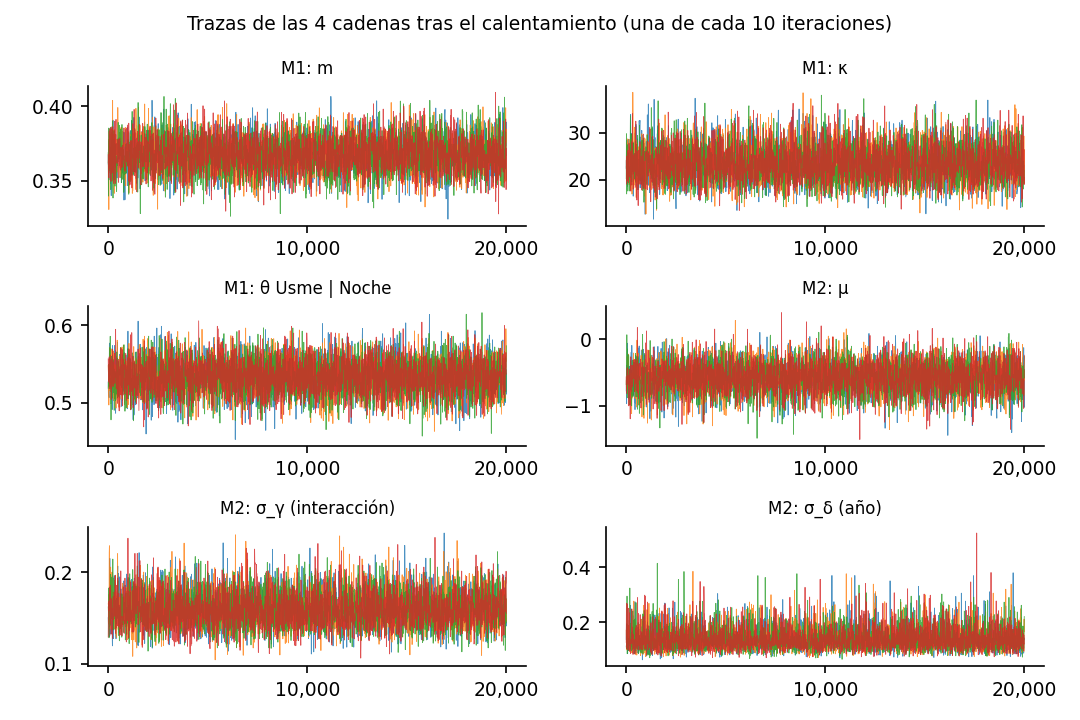
\includegraphics[width=\columnwidth]{figuras/trazas.png}
\caption{Trazas de las cuatro cadenas (colores) para parámetros representativos de M1 y M2. Se mezclan alrededor del mismo valor desde el inicio: no hay evidencia de falta de convergencia. Fuente: elaboración propia con datos de la SDM \citep{sdm2021datos}.}\label{fig:trazas}
\end{figure}
\begin{figure}[t]
\centering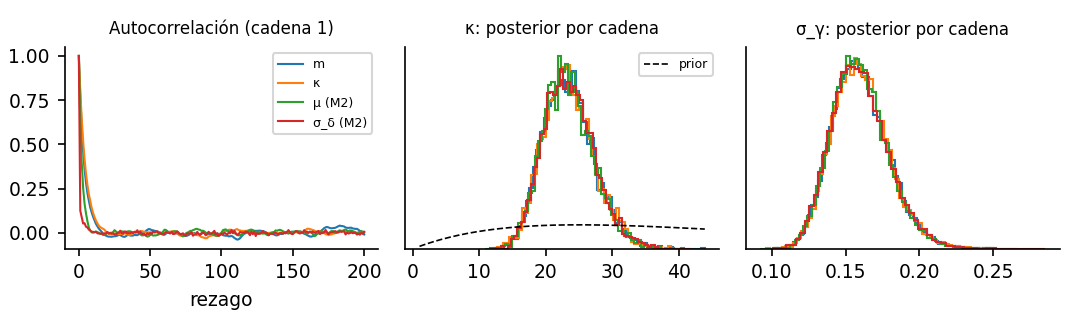
\includegraphics[width=\columnwidth]{figuras/autocorr_densidades.png}
\caption{Izquierda: autocorrelación de la cadena 1. Centro y derecha: densidad posterior de $\kappa$ (con su prior punteada) y de $\sigma_g$ por cadena; las cuatro coinciden. Fuente: elaboración propia con datos de la SDM \citep{sdm2021datos}.}\label{fig:acf}
\end{figure}

\subsection{Estimaciones posteriores}
\textbf{M1.} La severidad típica de una celda es $m=36{,}7$\,\% (IC 90\,\%: 34,9--38,6) y la ciudad ``presta'' $\kappa=23$ siniestros (17,7--30,1) a cada celda: una celda con 23 siniestros queda a mitad de camino entre su proporción y la de la ciudad, y una con 500 conserva el 96\,\% de su propia proporción. La posterior de $\kappa$ quedó muy por debajo de la media de la prior (50) y no cambió al centrar la prior en 10 o en 300 (Tabla~\ref{tab:sens}): los datos dominan.

\textbf{M2.} La variación entre localidades ($\sigma_a=0{,}43$; 0,33--0,55) y entre franjas ($\sigma_b=0{,}37$; 0,25--0,56) es mayor que la interacción ($\sigma_g=0{,}16$; 0,13--0,19), lo que confirma la estructura casi aditiva de la EDA. Frente a la franja promedio, la razón de odds es 1,14 (1,08--1,21) en la noche, 1,09 (1,02--1,16) en la madrugada, 0,95 (0,90--1,01) en la mañana y 0,84 (0,80--0,89) en la tarde. El nivel anual varía con $\sigma_d=0{,}14$ (0,09--0,22): 2015 fue más severo ($d=+0{,}14$) que 2016 ($-0{,}05$) y 2017 ($-0{,}09$).

\textbf{Agrupamiento parcial.} En las celdas con al menos 30 siniestros el ajuste más grande fue de 4,5 puntos (Figura~\ref{fig:enc}); las celdas grandes casi no se mueven. M2 acerca las celdas pequeñas a lo que dicen su localidad y su franja, no al promedio de toda la ciudad como M1, y por eso las mueve menos hacia el centro cuando pertenecen a una localidad severa. Los órdenes de M1 y M2 coinciden en $\rho=0{,}99$.

\textbf{Qué pasa en una celda.} En Rafael Uribe Uribe en la noche hubo $n_c=705$ siniestros en 2015--2017 (denominador) y $y_c=388$ graves (numerador): la proporción cruda es $388/705=55{,}0$\,\%. M1 le suma a la celda unos 23 siniestros con la severidad de la ciudad: $(0{,}367\cdot23{,}5+388)/(23{,}5+705)=54{,}4$\,\%. Como la celda es grande, casi no se mueve. M2 da 54,7\,\% (47,3--61,9), un valor parecido pero con un intervalo más ancho, porque incluye lo que puede variar un año nuevo. La diferencia entre modelos se ve en una celda pequeña: La Candelaria en la madrugada tuvo 8 graves de 23 (34,8\,\%). M1 la acerca al promedio de la ciudad (35,8\,\%); M2 la acerca a lo que indican su localidad y su franja y la deja en 32,7\,\% (24,1--42,2). Eso es lo que cambia al introducir predictores: la celda ya no se apoya en toda la ciudad, sino en las celdas que se le parecen.
\begin{figure}[t]
\centering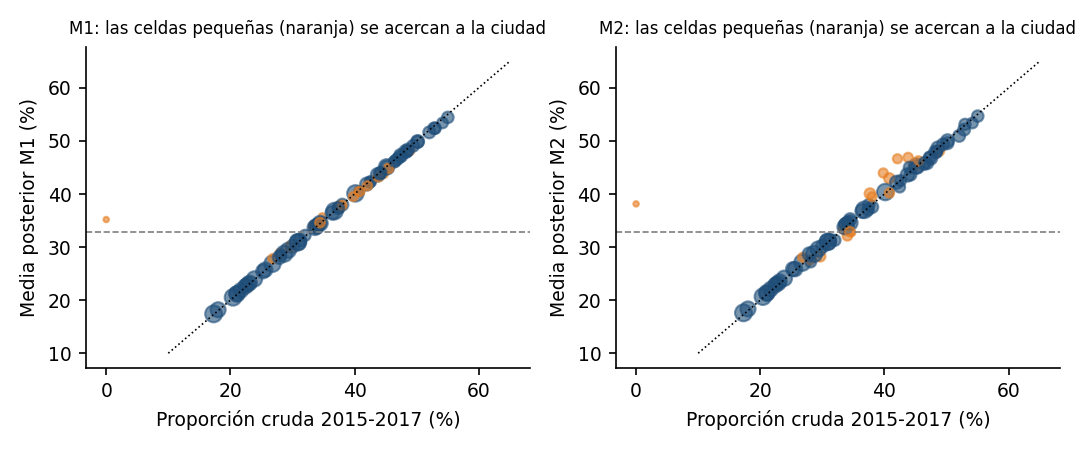
\includegraphics[width=\columnwidth]{figuras/encogimiento.png}
\caption{Proporción cruda 2015--2017 frente a la media posterior. El tamaño del punto es proporcional a $\sqrt{n_c}$; naranja: celdas con menos de 500 siniestros. La línea punteada es la identidad y la discontinua, el promedio de la ciudad. Fuente: elaboración propia con datos de la SDM \citep{sdm2021datos}.}\label{fig:enc}
\end{figure}

\subsection{Validación con 2018--2019}
La Tabla~\ref{tab:val} es la prueba principal, hecha una sola vez. Ambos modelos cumplieron los tres criterios de éxito a la vez. M2 obtuvo la mejor correlación de orden (0,933 frente a 0,921 de la proporción cruda y $-0{,}329$ del conteo), el menor Brier (0,22169 frente a 0,22181) y el menor log-loss, y empató en 6 coincidencias del top 10. La diferencia de Brier es pequeña: casi todo el error de cualquier método viene de que la ciudad pasó de 32,8\,\% a 36,1\,\% de graves entre periodos (Figura~\ref{fig:anio}); si se corrige ese cambio de nivel, la proporción cruda y M2 quedan iguales (0,2209). El orden, que es lo que se usaría para priorizar, no depende de ese nivel.
\begin{table}[t]
\centering\small
\caption{Desempeño en 2018--2019 (75 celdas con $\ge30$ siniestros en ambos periodos para el orden; todos los siniestros para Brier y log-loss, LogL). Más bajo es mejor en Brier y LogL; más alto en Spearman ($\rho$), top 10, lpd y cobertura del intervalo predictivo del 90\,\% (Cob.). Fuente: elaboración propia con datos de la SDM \citep{sdm2021datos}.}\label{tab:val}
\setlength{\tabcolsep}{2pt}\footnotesize
\begin{tabular}{@{}lcccccc@{}}
\toprule
Método & Brier & LogL & $\rho$ & Top10 & lpd & Cob. \\
\midrule
Conteo graves & -- & -- & $-0{,}329$ & 0 & -- & -- \\
Ciudad & 0,23175 & 0,6564 & -- & -- & -- & -- \\
Prop. cruda & 0,22181 & 0,6349 & 0,921 & 6 & -- & -- \\
M1 Beta-Bin. & 0,22179 & 0,6346 & 0,923 & 6 & $-430$ & 49\,\% \\
\textbf{M2 Logística} & \textbf{0,22169} & \textbf{0,6344} & \textbf{0,933} & 6 & $\bm{-375}$ & \textbf{95\,\%} \\
\bottomrule
\end{tabular}
\end{table}

La diferencia real entre los modelos está en la incertidumbre. Los intervalos predictivos del 90\,\% de M2 contuvieron el número observado de graves en el 95\,\% de las celdas; los de M1, solo en el 49\,\%. M1 no tiene efecto de año y trata 2018--2019 como si fuera igual a 2015--2017, así que es demasiado seguro de sí mismo; M2 incorpora la variación entre años mediante $d^{*}$ y por eso su densidad predictiva es mucho mejor ($-375$ frente a $-430$). Para declarar ``qué tan segura es cada cifra'', que es parte de la pregunta, M2 es el modelo adecuado.
\begin{figure}[t]
\centering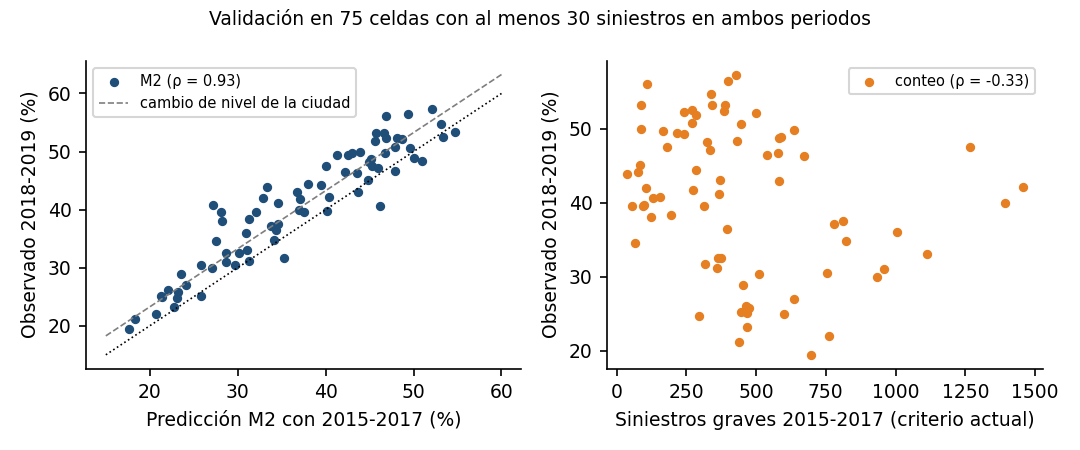
\includegraphics[width=\columnwidth]{figuras/validacion.png}
\caption{Izquierda: severidad predicha por M2 con 2015--2017 frente a la observada en 2018--2019; la nube sigue la línea discontinua (identidad desplazada por el cambio de nivel de la ciudad). Derecha: el criterio de conteo frente a la severidad observada; la relación es negativa. Fuente: elaboración propia con datos de la SDM \citep{sdm2021datos}.}\label{fig:val}
\end{figure}

\textbf{Equidad del error.} El MAE de M2 fue de 3,8 puntos en el sur frente a 4,3 en el resto, y de 4,6 en noche y madrugada frente a 3,7 en mañana y tarde: ninguna diferencia supera el umbral de 3 puntos. El sur no queda sobreestimado (sesgo de $-2{,}6$ puntos, subestimado como toda la ciudad por el cambio de nivel). Las celdas pequeñas sí encienden la alerta: MAE de 6,7 frente a 3,4 puntos (3,2 de diferencia). La mayor parte es azar del periodo de prueba: con pocos siniestros la proporción observada fluctúa, y solo por ese azar binomial se esperarían 3,0 y 1,3 puntos; el exceso sobre ese piso es de 3,7 frente a 2,2 puntos, una diferencia de 1,5. La cobertura de M2 en esas celdas fue de 87,5\,\%, cerca del 90\,\% nominal, y ninguna celda pequeña entra en la prioridad 1. Aun así, las 21 celdas pequeñas se entregan con su intervalo y no se ordenan por la media sola.

\subsection{Sensibilidades}
Las cinco sensibilidades definidas en el Avance 2 (Tabla~\ref{tab:sens}) muestran que el orden no depende de la prior de $\kappa$ y se mantiene con franjas de tres horas. Con solo siniestros con muertos la letalidad es más nocturna que territorial: las 10 celdas más letales son todas de madrugada o noche (6 del sur) y solo 2 coinciden con el top 10 de severidad; las dos medidas se correlacionan en 0,71. Esto matiza la lectura del sur: allí se concentran los heridos, pero la muerte vial se concentra de noche en toda la ciudad. En 2020, con la pandemia, el orden de M2 todavía se correlacionó en 0,81 con lo observado, mientras el conteo dio $-0{,}37$. La caída frente a 0,93 es coherente con lo que \citet{soltani2023road} reportan en Adelaida durante el confinamiento, donde los puntos críticos y los días con más siniestros cambiaron.
\begin{table}[t]
\centering\small
\caption{Sensibilidades definidas en el Avance 2 (Spearman con el periodo de prueba). Fuente: elaboración propia con datos de la SDM \citep{sdm2021datos}.}\label{tab:sens}
\setlength{\tabcolsep}{3pt}
\begin{tabularx}{\columnwidth}{@{}Xccc@{}}
\toprule
Variante & $\rho$ modelo & $\rho$ cruda & Top10 \\
\midrule
M1, $\kappa$ con media 10 & 0,923 & 0,921 & 6 \\
M1, $\kappa$ con media 300 & 0,923 & 0,921 & 6 \\
M1, franjas de 3 h (149 celdas) & 0,906 & 0,902 & 5 \\
M1, solo con muertos & 0,845 & 0,842 & -- \\
M2 frente a 2020 (74 celdas) & 0,807 & 0,834 & 3 \\
\bottomrule
\end{tabularx}
\end{table}

\subsection{Respuesta a la pregunta de investigación}
La probabilidad de que un siniestro sea grave cambia por un factor de tres entre celdas: de 17,6\,\% (IC 90\,\%: 13,8--21,9) en Usaquén en la tarde a 54,7\,\% (47,3--61,9) en Rafael Uribe Uribe en la noche (Figura~\ref{fig:top}). El cambio se explica sobre todo por la localidad y luego por la franja: las 24 celdas de las seis localidades del sur están, con más de 95\,\% de probabilidad, por encima del promedio de la ciudad, y la noche y la madrugada son más severas en casi todas partes.

Con qué seguridad: 9 celdas tienen probabilidad posterior de al menos 50\,\% de estar en el top 10 (5 de ellas por encima de 90\,\%), 7 más tienen entre 10\,\% y 50\,\%, y las 5 celdas con menos de 30 siniestros (Sumapaz y La Candelaria en la madrugada) son no concluyentes. Para la SDM proponemos tres niveles en lugar de un ranking de 80 puestos: \emph{prioridad 1}, las 9 celdas con $P(\text{top 10})\ge0{,}5$; \emph{prioridad 2}, las otras 32 celdas por encima del promedio con más de 95\,\% de probabilidad; y \emph{seguimiento}, el resto.
\begin{figure}[t]
\centering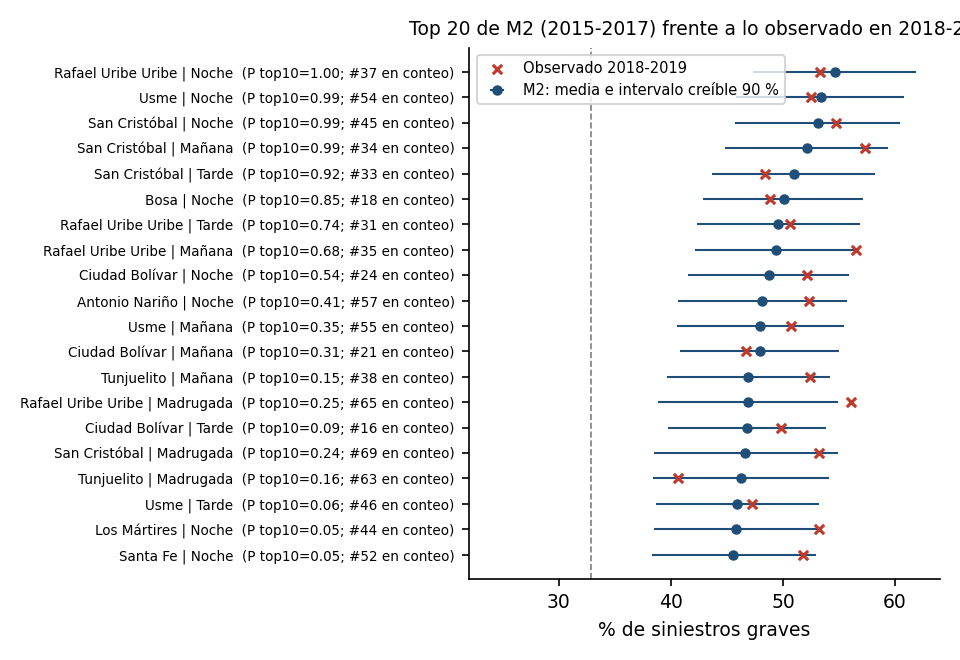
\includegraphics[width=\columnwidth]{figuras/top20_forest.png}
\caption{Las 20 celdas más severas según M2: media e intervalo creíble del 90\,\% para un año nuevo (incluye la variación entre años), probabilidad de estar en el top 10 y puesto en el orden por conteo. Las cruces son lo observado en 2018--2019. Fuente: elaboración propia con datos de la SDM \citep{sdm2021datos}.}\label{fig:top}
\end{figure}

Cuánto cambia el orden: por completo. Ninguna de las 10 celdas prioritarias de M2 está entre las 10 con más siniestros graves; en el orden por conteo ocupan los puestos 18 a 57. A la inversa, las 10 celdas con más graves (Kennedy, Engativá, Suba y Puente Aranda, sobre todo en la mañana y la tarde) quedan entre los puestos 21 y 67 por severidad. Los dos órdenes se correlacionan en $-0{,}19$, y en el periodo no visto el conteo apuntó en la dirección contraria a la severidad ($\rho=-0{,}33$) mientras el modelo acertó ($\rho=0{,}93$). En la práctica, con capacidad para 10 celdas, las 10 de M2 tuvieron en 2018--2019 6.048 siniestros con 52,4\,\% de graves, y las 10 del conteo 21.016 con 36,9\,\%, casi el promedio de la ciudad (36,1\,\%). Ordenar por conteo lleva a donde se acumulan más siniestros, no a donde los siniestros dejan más víctimas. La severidad complementa a la concentración; no la reemplaza, porque una celda con muchos siniestros sigue sumando muchas víctimas aunque su proporción sea baja.

\subsection{Discusión}
El modelo aporta poco sobre la proporción cruda en el orden de las celdas grandes: casi todas tienen cientos o miles de siniestros y el agrupamiento parcial apenas las mueve. Es lo mismo que sugiere la literatura: \citet{lim2013identifying} encontraron que el conteo simple funciona bien en el extremo superior, y la ventaja de los métodos bayesianos aparece sobre todo con pocos datos. El aporte del modelo está en tres cosas que la regla simple no da: un intervalo calibrado para cada celda (cobertura de 95\,\% frente a 49\,\% de M1), una probabilidad de estar entre las prioritarias, que dice qué posiciones son firmes y cuáles no, y estimaciones más estables en las celdas pequeñas (MAE de 6,7 puntos frente a 7,5 de la cruda y de M1).

Frente a otros estudios, la relación negativa entre concentración y severidad que encontramos ($-0{,}63$ por localidad y $-0{,}19$ por celda) es coherente con la idea de \citet{stipancic2019network} de que frecuencia y severidad son dimensiones distintas. Que la franja importe y que su efecto cambie un poco según la localidad ($\sigma_g=0{,}16$) va en la línea de \citet{zeng2023bayesian} y \citet{zou2017truck}, que encontraron diferencias entre el día y la noche en los factores y en la severidad, aunque en otros contextos y con flujo vehicular. Y el peso de la localidad es coherente con que en Colombia la gravedad se asocie con factores del entorno, como la velocidad permitida o la infraestructura \citep{cantillo2020exploratory,vergel2020examining}, que nuestra base no trae.

Hay cuatro límites. Primero, no pudimos confirmar con qué criterio reparte hoy la SDM sus operativos por zona y hora (no hubo contacto con la entidad; el siguiente paso es un derecho de petición). Sus tramos críticos publicados se definen por concentración de víctimas \citep{sdm2026tramos}, lo que es coherente con la referencia de conteo que usamos, pero a otra escala; si la SDM prioriza de otra forma, la comparación cambia de objeto. Segundo, la severidad no es riesgo: sin exposición no sabemos cuántos siniestros \emph{debería} haber en cada celda. Tercero, la mayor severidad del sur puede reflejar en parte que allí se reportan menos los choques leves; la sensibilidad con muertos muestra que la letalidad es sobre todo nocturna ($\rho=0{,}71$ con la severidad; 2 de 10 celdas en común), así que nuestra afirmación se limita a la \emph{severidad registrada}. Cuarto, el periodo de prueba se miró en una versión temprana de la EDA y el Brier de referencia de la proporción cruda se calculó con esos mismos datos; desde entonces todo lo que alimenta los modelos usa solo 2015--2017. Ninguna celda debe usarse para evaluar el desempeño de agentes de campo: si el indicador se vuelve meta, puede cambiar la forma de registrar. Por último, los datos terminan en 2020: el resultado es un \emph{prototipo retrospectivo} que debe actualizarse con datos posteriores y validarse con la SDM antes de apoyar decisiones operativas.

% ------------------------------------------------------------------ 5
\section{Conclusiones}\label{sec:con}
(1) La severidad de los siniestros en Bogotá depende mucho de dónde y cuándo ocurren: va de 18\,\% a 55\,\% entre celdas, más por localidad que por franja. (2) Priorizar por severidad registrada y por conteo lleva a listas disjuntas; en un periodo no visto la primera acertó ($\rho=0{,}93$) y la segunda no ($\rho=-0{,}33$). (3) El modelo logístico jerárquico cumplió los tres criterios de éxito definidos antes de estimar y entregó intervalos calibrados, aunque su ventaja en el orden frente a la proporción cruda es pequeña; el Beta-Binomial ordena igual pero subestima la incertidumbre porque ignora la variación entre años. (4) Como prototipo retrospectivo, proponemos a la SDM usar los tres niveles de prioridad como segundo criterio junto al conteo, una vez actualizados los datos posteriores a 2020; en la severidad registrada, las celdas más claras son las noches del sur (Rafael Uribe Uribe, Usme, San Cristóbal, Bosa y Ciudad Bolívar) y San Cristóbal en todas sus franjas. El cuarto objetivo quedó a medias: tradujimos el resultado a niveles de prioridad y declaramos sus límites, pero no logramos presentarlo a la SDM. Como trabajo futuro: confirmar con la SDM su criterio actual y si usaría el resultado, actualizar los datos con la capa vigente de la SDM, añadir exposición (aforos) para pasar de severidad a riesgo y modelar por separado heridos y muertos.

\bibliographystyle{apalike_sf}
\bibliography{Bibliografia}

% ------------------------------------------------------------------ APÉNDICE
\appendix
\section{Apéndice matemático}\label{sec:apx}
\subsection{M1: condicional completa de $\theta_c$ (paso de Gibbs)}
Por la independencia condicional de las celdas,
\begin{align*}
p(\theta_c\mid m,\kappa,\bm y)&\propto \theta_c^{y_c}(1-\theta_c)^{n_c-y_c}\\
&\quad\times\theta_c^{m\kappa-1}(1-\theta_c)^{(1-m)\kappa-1}\\
&=\theta_c^{m\kappa+y_c-1}(1-\theta_c)^{(1-m)\kappa+n_c-y_c-1},
\end{align*}
es decir, $\theta_c\mid\cdot\sim\mathrm{Beta}(m\kappa+y_c,(1-m)\kappa+n_c-y_c)$.

\subsection{M1: media condicional y agrupamiento parcial}\label{apx:enc}
La media de esa Beta es
\begin{align*}
E[\theta_c\mid\cdot]&=\frac{m\kappa+y_c}{\kappa+n_c}=w_c\,m+(1-w_c)\frac{y_c}{n_c},\\
w_c&=\frac{\kappa}{\kappa+n_c}.
\end{align*}
El peso de la ciudad, $w_c$, va a 0 cuando $n_c\to\infty$ y a 1 cuando $n_c\to0$. Con $\kappa\approx23$: $w=0{,}5$ si $n_c=23$ y $w=0{,}044$ si $n_c=500$.

\subsection{M1: densidad de $(m,\kappa)$ y paso de Metropolis-Hastings}\label{apx:m1}
Dados $\bm\theta$, la condicional de $(m,\kappa)$ no depende de $\bm y$:
\begin{multline*}
p(m,\kappa\mid\bm\theta)\propto\prod_{c=1}^{80}\frac{\theta_c^{m\kappa-1}(1-\theta_c)^{(1-m)\kappa-1}}{B(m\kappa,(1-m)\kappa)}\\
\times m(1-m)^{3}\,\kappa e^{-0{,}04\kappa}.
\end{multline*}
Con $u=\logit m$, $v=\log\kappa$ el jacobiano es $|\partial(m,\kappa)/\partial(u,v)|=m(1-m)\kappa$, de modo que
\begin{multline}
\log\pi(u,v\mid\bm\theta)=\sum_c\big[(m\kappa-1)\log\theta_c\\
+((1-m)\kappa-1)\log(1-\theta_c)\big]-80\log B(m\kappa,(1-m)\kappa)\\
+2\log m+4\log(1-m)+2v-0{,}04\kappa+\text{cte.}\label{eq:apx_m1}
\end{multline}
La propuesta $q(u',v'\mid u,v)=N\big((u,v),\mathrm{diag}(s_u^2,s_v^2)\big)$ es simétrica, así que la probabilidad de aceptación es $\alpha=\min\{1,\pi(u',v')/\pi(u,v)\}$. Con ella se cumple el balance detallado, $\pi(x)q(x'\mid x)\alpha(x,x')=\pi(x')q(x\mid x')\alpha(x',x)$, y $\pi$ es la distribución estacionaria. Combinar este paso con el de Gibbs (que acepta siempre) deja invariante la posterior conjunta \citep[cap.~11]{gelman2013bda}. La escala solo se adapta durante el calentamiento, que se descarta.

\subsection{M2: pasos por componentes, traslaciones y varianzas}\label{apx:m2}
Sea $\ell_{lft}(\eta)=y_{lft}\eta-n_{lft}\log(1+e^{\eta})$ la log-verosimilitud binomial en la escala logit, con $\eta_{lft}=\mu+a_l+b_f+g_{lf}+d_t$.

\textbf{Factorización.} Dados los demás parámetros, $p(\bm a\mid\cdot)\propto\prod_l\big[\exp\{\sum_{f,t}\ell_{lft}\}\,N(a_l\mid0,\sigma_a^2)\big]$: cada $a_l$ es condicionalmente independiente de los otros. Proponer los 20 a la vez y aceptar cada uno con
\[
\log r_l=\sum_{f,t}\big[\ell_{lft}(\eta')-\ell_{lft}(\eta)\big]-\frac{a_l'^2-a_l^2}{2\sigma_a^2}
\]
equivale a 20 pasos MH secuenciales. Lo mismo vale para $b_f$ (suma sobre $l,t$), $g_{lf}$ (sobre $t$) y $d_t$ (sobre $l,f$).

\textbf{Traslaciones.} La propuesta $(\mu',\bm a')=(\mu+c,\bm a-c\bm 1)$, $c\sim N(0,s^2)$, deja $\eta$ intacto, así que la razón de verosimilitudes es 1 y
\[
\log r=-\frac{(\mu'-\mu_0)^2-(\mu-\mu_0)^2}{2}-\frac{\sum_l(a_l'^2-a_l^2)}{2\sigma_a^2}.
\]
Es simétrica y preserva la posterior; mueve la cadena a lo largo de la dirección mal identificada ($\mu$ frente a la media de los efectos) y explica el ESS alto de $\mu$.

\textbf{Varianzas (Gibbs).} Si $x_1,\dots,x_J\mid\sigma^2\sim N(0,\sigma^2)$ y $\sigma^2\sim\mathrm{IG}(\alpha,\beta)$,
\[
p(\sigma^2\mid\bm x)\propto(\sigma^2)^{-J/2}e^{-\sum x_j^2/2\sigma^2}(\sigma^2)^{-\alpha-1}e^{-\beta/\sigma^2},
\]
que es $\mathrm{IG}\big(\alpha+J/2,\ \beta+\tfrac12\sum_jx_j^2\big)$, con $J=20,4,80,3$ para $a,b,g,d$.

\subsection{Cantidades predictivas y métricas}
\textbf{Predicción.} Para cada iteración $s$: $\theta^{(s)}_{c}$ (M1) o $\theta^{\mathrm{nuevo},(s)}_{lf}=\expit(\mu^{(s)}+a_l^{(s)}+b_f^{(s)}+g_{lf}^{(s)}+d^{*(s)})$ con $d^{*(s)}\sim N(0,\sigma_d^{2(s)})$ (M2). La predicción puntual es $\hat p_c=\frac1S\sum_s\theta^{(s)}_c$ y la predictiva de la prueba es $\tilde y_c^{(s)}\sim\mathrm{Bin}(n_c^{\mathrm{prueba}},\theta_c^{(s)})$; la cobertura es la fracción de celdas con $y_c^{\mathrm{prueba}}$ entre los cuantiles 5 y 95 de $\tilde y_c$.

\textbf{Métricas.} Con $N=\sum_cn_c$ siniestros de prueba,
\begin{align*}
\mathrm{Brier}&=\tfrac1N\textstyle\sum_c\big[y_c(1-\hat p_c)^2+(n_c-y_c)\hat p_c^2\big],\\
\mathrm{LogL}&=-\tfrac1N\textstyle\sum_c\big[y_c\log\hat p_c+(n_c-y_c)\log(1-\hat p_c)\big],\\
\mathrm{lpd}&=\textstyle\sum_c\log\Big(\tfrac1S\sum_s\mathrm{Bin}(y_c\mid n_c,\theta_c^{(s)})\Big),
\end{align*}
$\rho$ es la correlación de Spearman entre $\hat p_c$ y $y_c/n_c$, y $P(\text{top 10})_c=\frac1S\sum_s\mathbb 1\{\mathrm{rango}(\theta_c^{(s)})\le10\}$.

\textbf{Momentos de las priors.} Beta(2,4): media 1/3; Gamma(2;\,0,04): media 50; IG$(\alpha,\beta)$: media $\beta/(\alpha-1)$, es decir, 0,25, 0,05 y 0,025.

\end{document}
